% XCircuit output "packet2.tex" for LaTeX input from packet2.eps
\def\putbox#1#2#3#4{\makebox[0in][l]{\makebox[#1][l]{}\raisebox{\baselineskip}[0in][0in]{\raisebox{#2}[0in][0in]{\scalebox{#3}{#4}}}}}
\def\rightbox#1{\makebox[0in][r]{#1}}
\def\centbox#1{\makebox[0in]{#1}}
\def\topbox#1{\raisebox{-0.60\baselineskip}[0in][0in]{#1}}
\def\midbox#1{\raisebox{-0.20\baselineskip}[0in][0in]{#1}}
   \scalebox{1}{
   \normalsize
   \parbox{11.5in}{
   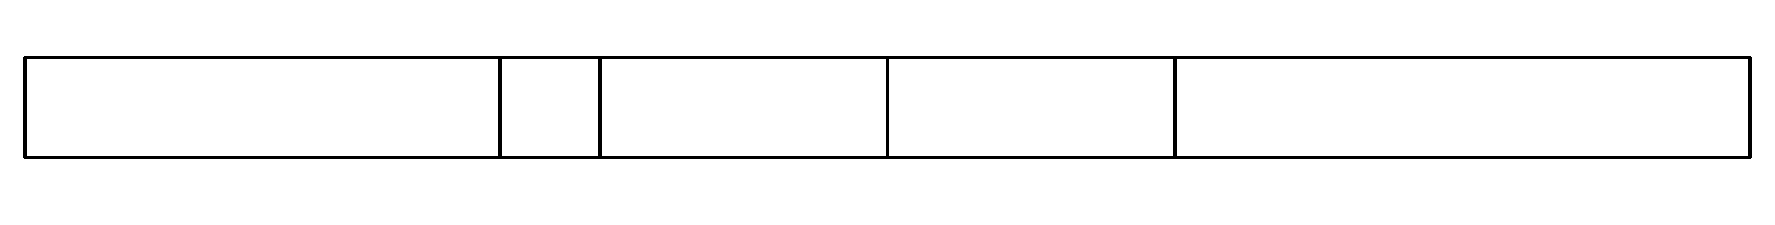
\includegraphics[scale=1]{packet2.eps}\\
   % translate x=1696 y=150 scale 0.38
   \putbox{4.06in}{1.09in}{1.20}{31}%
   \putbox{5.89in}{1.09in}{1.20}{23}%
   \putbox{7.89in}{1.09in}{1.20}{15}%
   \putbox{11.31in}{1.09in}{1.20}{0}%
   \putbox{4.47in}{0.09in}{1.20}{length}%
   \putbox{6.39in}{0.09in}{1.20}{op-code}%
   \putbox{9.14in}{0.09in}{1.20}{command}%
   \putbox{7.39in}{1.09in}{1.20}{16}%
   \putbox{5.39in}{1.09in}{1.20}{24}%
   \putbox{3.39in}{1.09in}{1.20}{32}%
   \putbox{3.31in}{0.09in}{1.20}{valid}%
   \putbox{2.97in}{1.09in}{1.20}{33}%
   \putbox{0.06in}{1.09in}{1.20}{63}%
   \putbox{1.14in}{0.09in}{1.20}{unused}%
   } % close 'parbox'
   } % close 'scalebox'
   \vspace{-\baselineskip} % this is not necessary, but looks better
